\section{Servizi di Cartografia}
Lo scopo del progetto richiede necessariamente il recupero e la manipolazione di dati cartografici, in particolare le mappe stradali e i possibili percorsi pedonali. Già dalle prime fasi del progetto, si è quindi presentata la necessità di individuare un servizio di cartografia da cui recuperare questi dati ed eventualmente sfruttare per la successiva manipolazione. I criteri di preferenza in questa scelta sono stati ancora una volta la facilità di accesso al servizio in termini di licenza, la diffusione e la documentazione disponibile.
Le due soluzioni che si sono prospettate sono i maggiori ``player'' in questo ambito, lasciando poco spazio ad altre opzioni in termini di compltezza dei dati e strumenti di integrazione. Si riassumono gli aspetti principali ed in particolare le differenze tra i due servizi che hanno determinato la scelta finale.

\subsection{Google Maps}
\begin{figure}[ht]
  \centering
  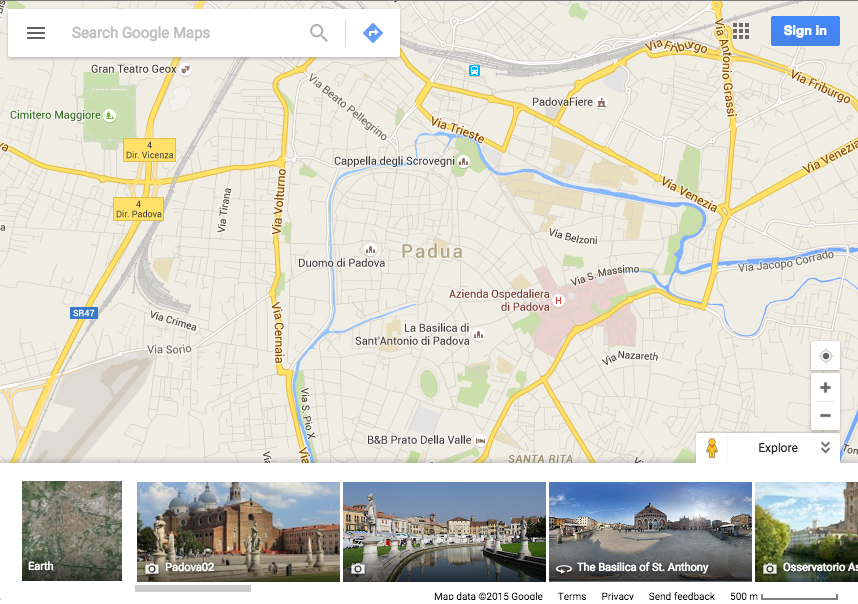
\includegraphics[width=\textwidth]{google-maps}
  \caption{\footnotesize{Schermata di accesso al servizio \emph{Google Maps}.}}
  \label{fig:google-maps}
\end{figure}
E' stato uno dei primi sevizi di mappe accessibili sul web, fin dall'Ottobre 2005. Negli anni si è evoluto profondamente sia in termini di completezza e accuratezza dei dati disponibli, che in termini di funzionalità e strumenti di interrogazione. Tramie Google Maps oggi è possibile accedere alle mappe stradali di tutto il mondo, percorsi pedonali, siti naturalistici, edifici pubblici di interesse, viste in prima persona e molto altro. Sono inoltre disponibili diversi strumenti per gli sviluppatori che consentono di accedere ai servizi basati su questi dati. La valutazione si è quindi concentrata sulla tipologia degli strumenti disponibili e sulle operazioni che sarebbe stato possibile eseguire (\url{https://developers.google.com/maps}).
Goggle fornisce \emph{API} e \emph{SDK} per le principali piattaforme applicative, sia \emph{desktop} che \emph{mobile}. Considerato però l'ambito specifico di utilizzo nel server \emph{PathS}, le funzionalità considerate sono quelle denominate \texttt{Web Services} ovvero interrogazioni \emph{HTTP} con risposte in formato \emph{JSON}. La prima caratteristica per cui si contraddistingue il servizio Google Maps è che non consente l'accesso diretto alle informazioni cartografiche. Non è possibile estrapolare parte di questi dati, siano essi in forma grezza o finita. Da qui la necessità di utilizzare uno dei servizi a disposizione per ottenere le informazioni necessarie, in particolare il servizio \textbf{Google Maps Direction API}. Con tale servizio è possibile ottenere un percorso impostando un punto di partenza ed una destinazione. Lo stesso servizio era utilizzato in precedenza dal progetto \emph{Path 2.0} e veniva impiegato direttamente per il calcolo della soluzione finale da proporre agli utenti. Tuttavia questo tipo di accesso non consente di ottenere dati per una determinata zona se non con una precisa interrogazione. Inoltre l'utilizzo delle \emph{API} presenta i seguenti limiti:
\begin{itemize}
\item il numero di interrogazioni è limitato dal tipo di piano utilizzato. Il servizio libero e gratuito denominato \emph{Standard} consente 2,500 chiamate al giorno, applicando una tariffa per le successive. Questa situazione sarebbe stata sostenibile per le prime fasi prototipali del progetto, ma non per una sua applicazione su larga scala.
\item il piano di utilizzo \emph{Standard} limita anche l'utilizzo delle funzione ``waypoint'' nel calcolo del percorso a 8 tappe intermedie. Questo risulterebbe un ulteriore limite nel calcolo dei percorsi complessi;
\item il servizio Maps opera direttamente sui dati memorizzati da Google ma non è possibile aumentare o integrare direttamente questo insieme di dati. Non è possibile quindi sfruttare gli algoritmi forniti dal servizio (es. calcolo percorso) su un insieme di informazioni \emph{custom} (es. i campioni di luminosità), se non tramite un uso indiretto e improprio delle \emph{API}.
\end{itemize}
Alla data in cui si è eseguita l'analisi comparativa, i servizi \emph{Google Maps} non disponevano ancora delle \emph{Roads API} introdotte in forma sperimentale nel Marzo 2015. La funzione di interpolazione e mapping dei punti GPS sarebbe risultata molto utile all'applicazione del progetto ma per questo motivo non è stata considerata.

\subsection{Open Street Map}
caratteristiche Open Street Map
\subsubsection
Il servizio di interrogazione \emph{Overpass API}, funzionalità e tipo di \emph{query} implementata.
\subsubsection
Mapquest

\section{Persistenza ed eleaborazione dei dati GIS}
Libreria scelta per la persistenza dei dati PostGIS, modello dati del DB e tipi utilizzati. Operazioni di interrogazione supportate dall'estensione del database.
Libreria scelta per la manipolazione dei dati in ambiente \emph{JAVA}:\emph{JTS}. Operazioni necessarie ed esempi di utilizzo. 

\section{Algoritmo di Map Matching}
Perchè è necessario eseguire una operazione di \emph{map matching}. A cosa servono questo tipo di algoritmi, panoramica sullo stato dell'arte e le soluzioni possibili.
\subsection{ST-MapMatching}
Esposizione delle caratteristiche principali dell'algoritmo come presentato in \cite{stmapmatching}.
\subsection{Pre-elaborazione del percorso - step 1}
Calcolo della bounding box, recupero della rete di trasporto coinvolta e inserimento a sistema.
\subsection{Identificazione dei candidati - step 2}
Definizione e modalità di calcolo dei candidati. Operazioni implementate ed esempi di esecuzione.
\subsection{Valutazione e selezione dei candidati - step 3}
Applicazione della valutazione spazio-temporale dei campioni. Algoritmo di selezione dei candidati da assegnare ai campioni. 